\PassOptionsToPackage{table}{xcolor}
\documentclass{beamer}
\usepackage{color}
\usepackage[color,matrix,arrow]{xypic}
\usepackage{tikz}
\usepackage{tikz-dependency}
\usepackage{tikz-qtree}
\usepackage{tkz-graph}
\usetikzlibrary{arrows,positioning}

\usetheme{default}

\begin{document}

\begin{frame}[fragile]
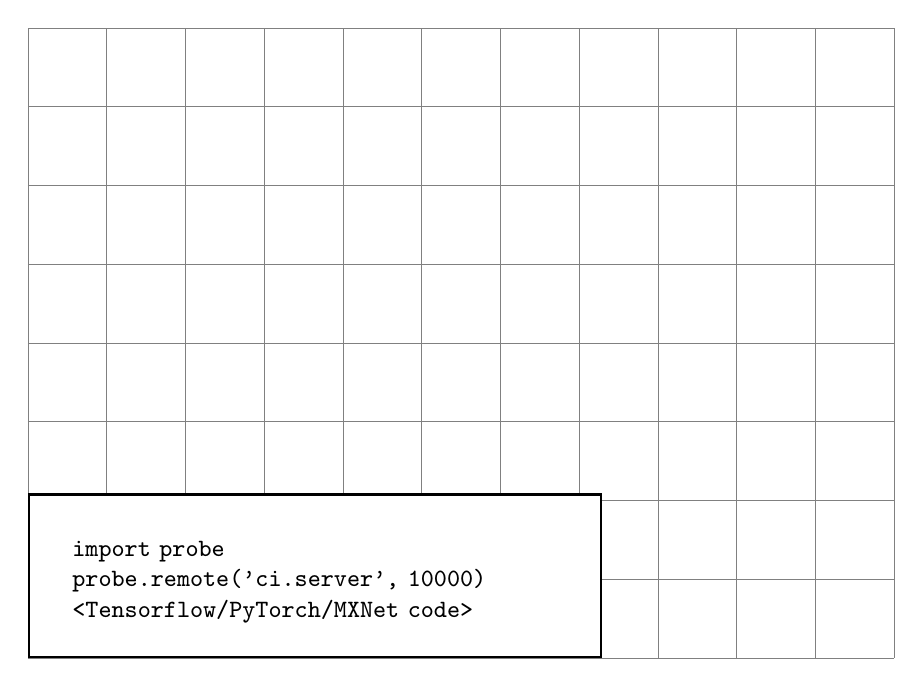
\begin{tikzpicture}[node distance=1cm, auto,
  ]
  %nodes
  \draw[help lines] (0,0) grid (11,8);
  \node at (0, 0) [anchor=south west, rectangle, draw=black, thick, fill=white, text width=20em, font=\small] (training) {
    \begin{verbatim}
    import probe
    probe.remote('ci.server', 10000)
    <Tensorflow/PyTorch/MXNet code>
    \end{verbatim}
  };

  %% %\node at (0, 0) [rectangle, draw=black, thick, fill=white, text height=20em, text width=12em] (ci_server) {
  %% %  CI server
  %% %};

  %% \node at (0, 8) [rectangle, draw=black, thick, fill=white, text width=12em] (visualization) {
  %%   Visualization
  %% };
  
  %\path[->, bend left=45] (training) edge node {Layer (serialized numpy array)} (ci_server);
  %\path[->, bend left=45] (ci_server) edge node {Plot} (visualization);

  
  
  % \node[inner sep=5pt,below=0.5cm of market]
% (formidler) {Intermediaries (c)};
 % We make a dummy figure to make everything look nice.
% \node[above=of market] (dummy) {};
% \node[right=of dummy] (t) {Ultimate borrower}
%   edge[bend left=45] (market.east) % edges are used to connect two nodes
%   edge[bend left=45] (formidler.east); % .east since we want
                                             % consistent style
% \node[left=of dummy] (g) {Ultimate lender}
%   edge[bend right=45] (market.west)
%   edge[bend right=45] (formidler.west)
%   edge[<->, bend left=45] node[auto] {Direct (a)} (t);
\end{tikzpicture}
\end{frame}


\begin{frame}[fragile]
  \frametitle{Setting up the server is a Docker container that exposes a REST endpoint}
\end{frame}

\begin{frame}[fragile]
Training DNN models:
\end{frame}

\begin{frame}[fragile]
Examining results:
\end{frame}

\end{document}
